\documentclass{beamer}
\usepackage{graphicx}

\title{Verified Metatheory and Type Inference for a Name-Carrying Simply-Typed $\lambda$-Calculus}
\author{Michael Rawson}
\date{Lent Term 2017}

\begin{document}
\frame{\titlepage}

\begin{frame}
\frametitle{Simply-Typed $\lambda$-Calculus}
\begin{align*}
M &::= x\ |\ \lambda \alert{(x : T)}.M\ |\ (M\ M)\\
T &::= T_0\ |\ T_1\ |\ \ldots\ |\ T \to T
\end{align*}

\begin{itemize}
\item $\lambda$-calculus, plus a na\"ive typing system
\item terms are familiar $\lambda$-terms, plus a \alert{typing annotation}
\item types are either a base type $T_n$ or a function type
\end{itemize}

However, $\alpha$-equivalence is a problem:
\begin{itemize}
\item would like to have $\lambda x.x = \lambda y.y$
\item surprisingly fiddly, many different approaches
\item unusual approach: ``can I swap names to make terms equal?''
\end{itemize}
\end{frame}

\begin{frame}
\frametitle{Progress}
\begin{center}
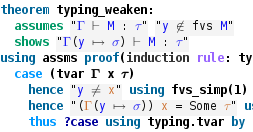
\includegraphics[width=0.5\textwidth]{screenshot}
\end{center}

\begin{itemize}
\item terms \emph{quotiented} with respect to $\alpha$-equivalence
\item typing and evaluation relations on these terms
\item metatheory: \emph{progress}, \emph{preservation}
\item verified type-inference algorithm
\item currrently refactoring and adding more metatheory
\end{itemize}
\end{frame}

\begin{frame}
\frametitle{Finish}
\end{frame}
\end{document}
